%%%%%%%%%%%%%%%%%%%%%%%%%%%%%%%%%%%%%%%%%
% Short Sectioned Assignment
% LaTeX Template
% Version 1.0 (5/5/12)
%
% This template has been downloaded from:
% http://www.LaTeXTemplates.com
%
% Original author:
% Frits Wenneker (http://www.howtotex.com)
%
% License:
% CC BY-NC-SA 3.0 (http://creativecommons.org/licenses/by-nc-sa/3.0/)
%
%%%%%%%%%%%%%%%%%%%%%%%%%%%%%%%%%%%%%%%%%

%----------------------------------------------------------------------------------------
%	PACKAGES AND OTHER DOCUMENT CONFIGURATIONS
%----------------------------------------------------------------------------------------

\documentclass[paper=a4, fontsize=10pt]{scrartcl} % A4 paper and 10pt font size

\usepackage[T1]{fontenc} % Use 8-bit encoding that has 256 glyphs
%\usepackage{fourier} % Use the Adobe Utopia font for the document - comment this line to return to the LaTeX default
\usepackage[english]{babel} % English language/hyphenation
\usepackage{amsmath,amsfonts,amsthm} % Math packages
\usepackage{lscape}
\usepackage{lipsum} % Used for inserting dummy 'Lorem ipsum' text into the template
\usepackage{courier}
\usepackage{url}
\usepackage{sectsty} % Allows customizing section commands
\setlength{\columnsep}{5mm}

\usepackage{geometry}
 \geometry{
 a4paper,
 total={170mm,257mm},
 left=20mm,
 top=20mm,
 }
 
 \usepackage{graphicx}
\graphicspath{ {images/} }

\usepackage{indentfirst}
\usepackage{dirtree}


\setlength\parindent{0pt} % Removes all indentation from paragraphs - comment this line for an assignment with lots of text

%----------------------------------------------------------------------------------------
%	TITLE SECTION
%----------------------------------------------------------------------------------------


\begin{document}


\begin{titlepage}

\newcommand{\HRule}{\rule{\linewidth}{0.5mm}} % Defines a new command for the horizontal lines, change thickness here

\center % Center everything on the page
 
%----------------------------------------------------------------------------------------
%	HEADING SECTIONS
%----------------------------------------------------------------------------------------

\textsc{\LARGE UCD Smurfit Graduate School of Business}\\[1.5cm] % Name of your university/college

\includegraphics[scale = 0.6]{images/logo.png} \\ [1cm]
\textsc{\Large Numerical Analytics and Software}\\[0.5cm] % Major heading such as course name

%----------------------------------------------------------------------------------------
%	TITLE SECTION
%----------------------------------------------------------------------------------------

\HRule \\[0.4cm]
{ \LARGE \bfseries Programming Assignment 2}\\[0.4cm] % Title of your document
\HRule \\[1.5cm]
 
%----------------------------------------------------------------------------------------
%	AUTHOR SECTION
%----------------------------------------------------------------------------------------

\begin{minipage}{0.4\textwidth}
\begin{flushleft} \large
\emph{Authors:}\\
\small{Eoghan \textsc{Aherne} (??? - MSc B.A Part-time) }\\
\small{Louis \textsc{Carnec} (??? - MSc B.A Part-time)}\\
\small{Conor \textsc{Reid} (16202630 - MSc B.A Part-time)}\\
\end{flushleft}
\end{minipage}
~
\begin{minipage}{0.4\textwidth}
\begin{flushright} \large
\emph{Lecturer:} \\
\small{Dr. Sean \textsc{McGarraghy}} % Supervisor's Name
\end{flushright}
\end{minipage}\\[4cm]

% If you don't want a supervisor, uncomment the two lines below and remove the section above
%\Large \emph{Author:}\\
%John \textsc{Smith}\\[3cm] % Your name

%----------------------------------------------------------------------------------------
%	DATE SECTION
%----------------------------------------------------------------------------------------
\vspace{3cm}
{\large \today}\\[1cm] % Date, change the \today to a set date if you want to be precise

\vfill % Fill the rest of the page with whitespace

\end{titlepage}

%----------------------------------------------------------------------------------------
%	MAIN BODY
%----------------------------------------------------------------------------------------
%\setlength{\parindent}{10ex}
%Context
\tableofcontents
\clearpage
\onecolumn
\section{Introduction}
\clearpage
\section{Theory}

\subsection{Overview}

\subsection{Questions}
useful to check for convergence of the residual to zero?\\
what matrix norms might be useful and why?\\
scaling be helpful?\\
which matrices do you get expect convergence and which do not? why?\\
effect of different values of tolerance?\\
effect of an ill-conditioned matrix?\\

\subsection {Business Applications}

Successive over-relaxation methods were preceded by the Gauss-Seidel algorithm developed in the 19\textsuperscript{th} century which enabled him to solve singular linear systems with equal numbers of unknowns and equations. Over-relaxation techniques later evolved with the work of David Young, these would enable systems of over 20,000 unknowns to be solved by 1965 \cite{saad2000iterative}. Such methods were initially used for systems with elliptic partial differential equations discretised with finite difference techniques (or multi-grid methods). 

A range of applications could benefit from the lower computational cost and memory requirements of these iterative methods. Specifically the SOR iterative method is beneficial in circuit analysis, quantitative finance and weather forecasting.
\subsection {SOR}
{The first part of our solution  deals with simply applying the successive over-relaxation (SOR) algorithm to a system of linear equations in the form $\textbf{A}\textbf{x} = \textbf{b}$. This is in an effort to solve for $x_{1\times n}$ given $A_{n\times n}$ and $b_{1\times n}$. One approach to solving this type of problem is to decompose A into its diagonal component ({\it D}), and upper and lower triangular components ({\it L} and {\it U}). This yields an expression on which the SOR, an iterative technique, can work and eventually solve. It should be noted that SOR is a modification of the Gauss-Seidel method, increasing the reaction factor from $\omega = 1$ to $\omega > 1$. The purpose of the relaxation factor is to modify the spectral radius (the largest eiganvalue) of the resulting matrix and thus cause convergence more quickly. In theory by increasing this factor, convergence should be positively affected. \\\\
It has been shown that the optimal value of $\omega$ can be expressed as
\begin {equation}
\omega^* = \frac{2}{1 + \sqrt{1 - r_\theta}(C)}
\end {equation}
where $C = -(D + L)^{-1}U$ (D, L and U as above). However, in general the finding of this optimal relaxation factor is more challenging and computational expensive than the system of linear equations that are to be solved. For this reason, $\omega$ in the range $1 \leq \omega^* \leq 2$ is chosen.\\\\
Taking into account the triangular nature of D, L and U $x^{k+1}$ (that is, x at the $k+1$ iteration of x) can be expressed as
\begin{equation}
x_{i}^{(k+1)} = (1 - \omega)x_{i}^{(k)} + \frac {\omega}{a_{ii}}\bigg( b_i - \sum\limits_{j<i} a_{ij} x_j^{k+1} - \sum\limits_{j>i} a_{ij}  x_j^{k} \bigg) , i = 1,2,......n
\end{equation}
Using the equation above it is possible through iteration to approximate the solution of $\textbf{A}\textbf{x} = \textbf{b}$.}
\subsection {Black-Scholes(-Merton)}

The Black-Scholes model provides a way to calculate option prices from stock prices. The Black-Scholes(-Merton) equation, based on the It\^{o} process ($dS = \mu S dt+ S$)

The implementation of the Black-Scholes-Merton pricing problem found in the module \texttt{tridiagM.py} takes advantage of the fact that the Black-Scholes differential equation as a system of linear equations ($\textbf{A}\textbf{x} = \textbf{b}$) can be written as a tridiagonal $(N-1)\times(N-1)$ matrix. This tridiagonal matrix, $\textbf{A}$, which by definition is a sparse matrix, can be solved using the Sparse SOR algorithm
 which solves for vector $\textbf{x}$ the system of linear equations $\textbf{A}\textbf{x} = \textbf{b}$ by successive iteration. 

We are able to approximate all option prices for a given stock price for all $m \in M$ by approximating the previous time step using a system of linear equations. There are two approximation in finding option prices for all time steps $m$. 

The first of these entails approximating put option prices at time $T$ given Stock prices and a known put option strike price, $X$. Using this approximation for $f_{n,M}$, we can solve the system of linear equation for option prices at previous time periods $f_{n,m}$.

Given that the matrix $\textbf{A}$ represents the finite difference constants relating $f_{n, m-1}$ to $f_{n, m-1}$ and that we can approximate the $N$ European put option prices at $f_{n,M}$, where $M=T$ and time at which the option is at maturity, given the fact that the portfolio must 

$P = -f + \frac{\partial{f}}{\partial{S}}S$
$\left( -\sigma S \frac{\partial{f}}{\partial{S}} +\sigma S \frac{\partial{f}}{\partial{S}} \right) dz = 0 $

 
\subsubsection{Creating the Grid}
To solve for option prices at all time steps we need create a grid of stock prices (S, the stock price vector) and of M time steps until maturity (T).
Options have expiration dates or maturity. For example, an option expires in 12 days (T=12) and since our time steps is days ($k=T/M=1$), there are $M=12$ grid steps. If our time step was half a day (k=0.5) for the same expiry date (12 days), the grid would have 24 time steps ($M = 12 \times 0.5$).
Stock prices can be any non-negative real number. However the grid must start at 0 since the put option price is the strike price when the stock price is zero ($f_{0,m} = X$). To use the Sparse SOR algorithm we must have a square matrix A. Therefore there must be the same number of grid steps for the time (M) and stock price (N) vectors (N=M).

A function (\texttt{createSandT}) was created to return two vectors for stock prices and times. The grid step lengths, $k$ (step length between time steps) and $h$ (step length between stock prices) are calculated from input parameters. $h$ is the length of the stock price divided by the number of time steps (M), $\frac{S_{max} - S_{0}}{M}$.

\subsubsection{Components of the system}
The triadiagonal matrix $\textbf{A}$ requires the length of $S$ and $t$ to initiate the length of the three diagonals which make up the matrix. The function \texttt{abcArrays} creates three arrays for the diagonals using a \texttt{for} loop. The arrays are referred to as; b (the main diagonal), a (the first diagonal below b), and c (the first diagonal above b). They are then passed to the \texttt{tridiag} function which returns the tridiagonal matrix $\textbf{A}$. We are able to build this matrix solely based on vectors S and t which gives us the number of steps in each direction since the components of the diagonals increase linearly with each time step. 

The first b vector of future prices at time T needs to be approximated. \texttt{vectorB} creates an array of zeros of length equal to the number of points in the S vector. The array is filled using a \texttt{for} loop which approximates the $n$ option prices at M ($f_{n,M}$) by calculating $X - ih$ where $i$ is looped, the option price is equal to $X - ih$ if it is positive and 0 if not, $max \{ X - nh, 0 \}$.

\subsubsection{Approximating 'past' option prices}

From the first option price approximation we can approximate all 'past' n option prices by looping through each time step backwards from $t=T$ to $t=0$ and solving the system of linear equations for $f$ at each step. The b vector approximated with \texttt{vectorB} is passed to the function \texttt{findPastOptionPrices}, and at each step the vector f ($f_{n,m}$) is approximated. This vector $f$ is then assigned to $b$ and the next time-step ($m-1$) is approximated.

The issue with this last function is that the Sparse SOR function is ran T times to calculate x for each time step. For large grids (large M) this results in long runtime.



\subsubsection{Finite Difference Method}





\subsection {Iterative algorithms / SOR}
\clearpage
\section{Code Base and Solution Design}
\subsection{SOR}
{There are a number of notable features of the solution given that are discussed here. 
An important design decision that was made here was to use compressed row storage (csr) for the input matrices. This is chosen as the optimal storage method, due to the nature of the input matrices having a small amount of non-zero entries. In traditional storage methods, each value in the matrix would be stored in memory making for quick access times for any one specific value. This requires $\Theta(n^2)$ storage space, which can cause issues with particularly large matrices. In contrast, csr only stores the non-zero entries, along with the location of that entity. While accessing the value of a given matrix coordinate is not as easy as with the traditional method, the storage required is $O(2t + n)$. This is significantly less, and thus clearly an optimal design choice.       \\\\
The \texttt{main.py} module, from where the program as a whole is instigated and controlled, first handles file input and output. By default, an \texttt{input.in} file is read from. This file is stored in the {\bf docs/} folder, and contains the dimension of the input A, A itself and b all in plain text in array format. On read, these matrices are converted to compressed row storage (csr) for optimal storage and performance. A python dictionary is created containing these elements. Also by default, a \texttt{nas\_SOR.out} file is used for logging purposes, stored too in the {\bf docs} folder. \\\\
It is possible however, to change these defaults and input another file stored locally elsewhere. This is achieved by specifying the path to this file as the first argument to the \texttt{main.py} module. Note, that both files with the '.in' and '.mtx' are acceptable input to the program. It is expected that the former be in the same format as that of the default input. However, '.mtx' files can contain a matrix already in csr format. This facilitates the use of matrices sourced from \url{http://math.nist.gov/MatrixMarket/}. In addition, it is possible to provide a second argument to the \texttt{main.py} module specifying the location of the new log file. This will have no effect on the contents of the logs, only the location where they are saved. \\\\
Once the input and output files have been handled, a number of checks are carried out on the input matrices. Firstly, a check is made for any zeros on the main diagonal of the {\bf A} matrix. From equation (1), it is clear that a divide-by-zero would occur should there be any zeros on the main diagonal of A, in the $\frac{\omega}{a_{ii}}$ term. \\\\
Next, a check is made for diagonal dominance of the {\bf A} matrix. A condition for the convergence on a solution of {\bf x} is that that matrix have a $r_\sigma (C) < 1$ for 
\begin{equation}
C = -(D + L)^{-1}U
\end{equation}
where D, L and U are as described earlier. Having said this, it is appropriate to check for row or column diagonal dominance, and thus sufficiently meet the above criteria. There are two separate methods in the \texttt{doMath.py} module to achieve this, using differing methodologies. The \texttt{isStrictlyDiagDom} method uses {\it for} loops, and returns the count of instances where diagonal dominance is violated. The \texttt{isStrictlyDiagonallyDominant} method on the other hand, takes advantage of the ability in {\it numpy} to find the sum of a matrix along each axis. The value on the diagonal is then removed from this sum, and checked against the new sum to check for dominance of that diagonal value. }
\subsection{Black-Scholes(-Merton)}


\subsection {Version Control}
{It was decided to make use of source control, specifically GitHub, to manage the collaboration and multi-developer aspect of this project. The public repository for the current solution is available at the following url \url{https://github.com/ReidConor/Sparse-SOR/tree/master/}. This contains just just the code used to achieve the solution outlined here, but also the source code for this paper as well as the test matrices and resulting logs used throughout. In addition, this repository provides posterity and a way to retrieve the source code in addition to the files provided in the submission of this paper.}
\subsection {Project Structure}
{Here, a brief discussion of the source code structure is included for reference. Spare-SOR is the name of the project, with the \texttt{main.py} module directly underneath. This ensures ease of running, as well as better handling dependancies throughout the project.  }\\
\dirtree{%
.1 Sparse-SOR.
.2 Report.
.3 (latex files)...
.3 Report.pdf.
.2 core.
.3 doMath.py.
.3 fileIO.py.
.3 tridiagM.py.
.3 visualize.py.
.2 docs.
.3 Various .in files...
.3 Various .mtx files...
.3 Plots if generated...
.2 logs.
.3 BSM\_logs.out.
.3 nas\_SOR.out.
.3 Any other .out generated by providing an argument at runtime. 
.2 tests.
.3 outfile.txt.
.3 TestingC.py.
.3 tests.doc.
.3 unitTests.py.
.2 main.py.
.2 README.md.
}
\vspace{0.5cm}
{The {\it 'Report'} folder obviously contains this paper. The {\it core} folder contains much of the logic for SOR, as well as file input and output logic and methods for visualising results. The methods for solving the BSM equation is also found here. The {\it docs} folder contains the input matrices that were tested, and also provides a location to write plots out to if necessary. The {\it logs} folder obviously contains output files describing what happened in the latest run, and {\it tests} contains both unit testing and also methods used in the construction and running of tests for the SOR algorithm itself.}   
\subsection {Run Time}
{As mentioned previously, the \texttt{main.py} module controls the flow of the program, calling methods on the adjacent packages. Thus, it is this module that is run to invoke the functionality of the solution. Firstly, it is possible to run this module with no arguments. This will run the SOR algorithm against a default {\it '.in'} file containing a simple $5 \times 5$ matrix A and output the solution to the default logging location, a file called {\it nas\_SOR.out} in the \texttt {docs} folder.\\\\ Secondly, one can provide an argument when running the module. This would be the path to another data input file to solve using the SOR algorithm. Note, that this file can be in one of two forms; plain text or compress row storage. The former should be held in a {\it '.in'} file, the latter a {\it '.mtx'} file. This aids the program in deciding how best to treat the input, while allowing a diverse set of allowable input data. Passing a data file with a different file extension will cause the program to fail, and output 'input file error' in the logs.\\\\Thirdly, it is possible to pass a second parameter to the \texttt{main.py} module, which specifies a location in which to save the log file. This log file has been mentioned earlier, and simply provides a way to see what happened in the latest run of Sparse-SOR. Note, it is only possible to provide this alternative location if a path to the input file is also specified.    }
\subsection {Testing}
{Why testings important, how we found it really useful all the way through the assignment (lol). Brief overview of what tests we have included, maybe some specific problem we meet and how testing helped us solve it?}
\clearpage
\section{Technical Challenges and Limitations}
{What were the main technical challenges we faced doing this. What are the limitations of our brilliant solution }
\clearpage
\section{Results}
{Our fantastic results}

\subsection{Black-Scholes-Merton Results}

The number of grid points and thus the shape of the matrix depend on the values of M given. The program was run using a maturity of 12 months, a strike price of 100 and three different M values; M=12 for months, arbitrary M=40, and M=365 for days. The first three figures in Appendix 4.2 demonstrate the relationship between stock prices and option prices that satisfy the Black-Scholes equation. Each line from top to bottom represent a time step from T to 0 respectively. We can see that the distribution of the the put option prices vary greatly among the three figures. As $k$, the length between each time step decreases and the number of steps increases, the range of put option prices increases; the further the option is from maturity the lower its price. There is a reversal point in each figure which can only be spotted looking at the data in 2d, this is most obvious in the first two figures, the yellow line (option prices at time T) goes from being on top (option price is highest for some stock price $p$) to being on the bottom (option price is lowest for some stock price $p$). Therefore we can say that there is some threshold option price ($f^{*}_{n,m}$) and stock price ($p^{*}_{n,m}$) dependent on the time step ($m$) at which the slope of the curve decreases. From the 3D plots (figures 4,5 and 6), we can observe that the lower the value for k (the more steps maturity), the faster the fall in option price the further away from maturity and the greater the stock price.


\clearpage
\section{Conclusions}
\clearpage
\section*{Appendix}

\begin{figure}[h!]
\center
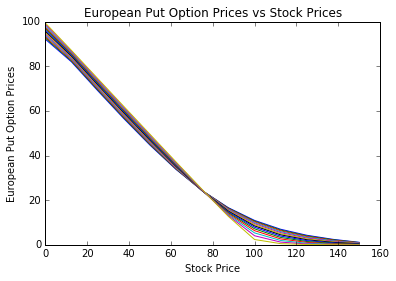
\includegraphics[scale=0.8]{vary1212.png}
\caption{Distribution of put option prices against stock prices for m $T=12$, $M=12$, $k=1$}
\end{figure}

\begin{figure}[h!]
\center
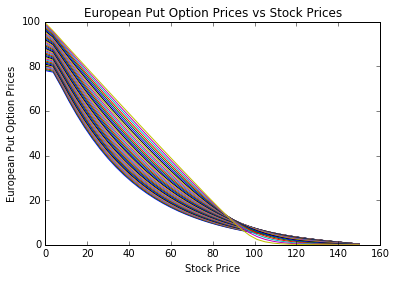
\includegraphics[scale=0.8]{vary1240.png}
\caption{Distribution of put option prices against stock prices for m $T=12$, $M=40$, $k=0.3$}
\end{figure}

\begin{figure}[h!]
\center
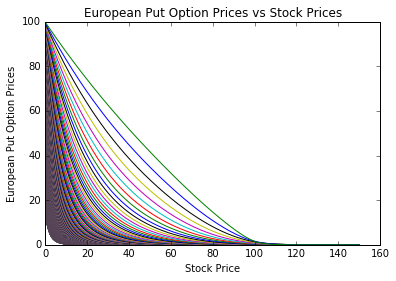
\includegraphics[scale=0.8]{vary12365.png}
\caption{Distribution of put option prices against stock prices for m $T=12$, $M=365$, $k=0.033$}
\end{figure}


\begin{figure}[h!]
\center
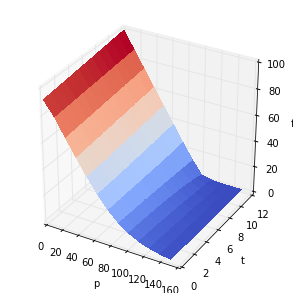
\includegraphics[scale=0.8]{3d_k_12_12.png}
\caption{3D Plot of European Put Option Prices for $T=12$, $M=12$, $k=1$}
\end{figure}

\begin{figure}[h!]
\center
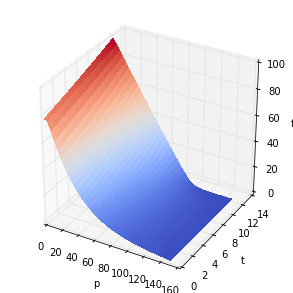
\includegraphics[scale=0.8]{3d_k_12_40.png}
\caption{3D Plot of European Put Option Prices for $T=12$, $M=40$, $k=0.3$}
\end{figure}

\begin{figure}[h!]
\center
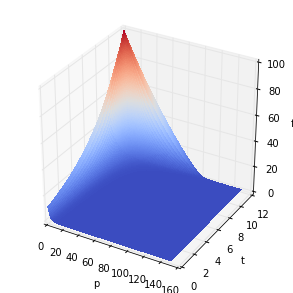
\includegraphics[scale=0.8]{3d_k_12_365.png}
\caption{3D Plot of European Put Option Prices for $T=12$, $M=365$, $k=0.033$}
\end{figure}


\clearpage
\begin{landscape}
\begin{figure}[h!]
\center
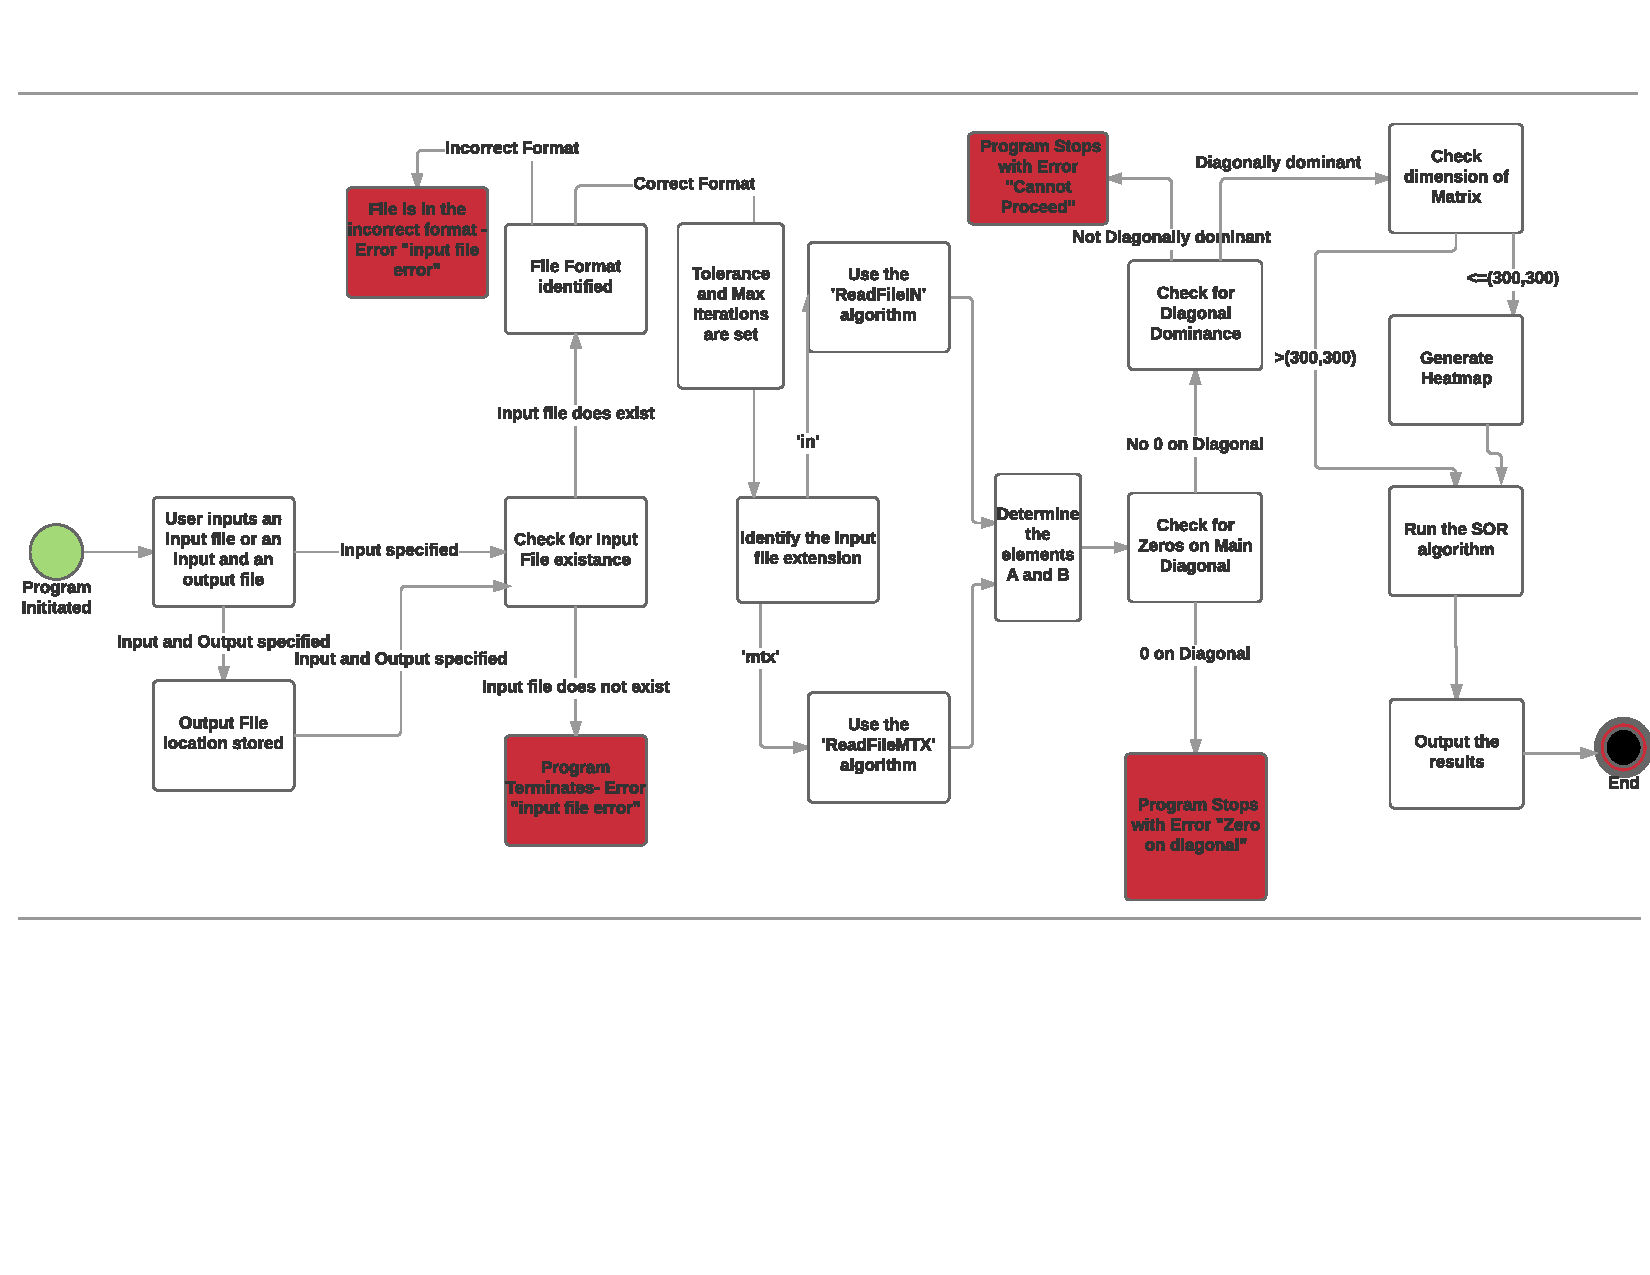
\includegraphics[scale=0.8]{NASprog.pdf}
\caption{Sparse SOR Application - Program Map}
\end{figure}
\end{landscape}

\clearpage
\bibliographystyle{acm}
\bibliography{numassignmentrefs}
 


\end{document}